\documentclass[aspectratio=169,11pt,t]{beamer}

% ============================================================
% Theme and typography
% ============================================================
\usetheme{Madrid}
\usecolortheme{default}
\usefonttheme{professionalfonts}
\setbeamertemplate{navigation symbols}{}
\setbeamertemplate{headline}{}
\setbeamertemplate{footline}{%
  \leavevmode\hbox{%
  \begin{beamercolorbox}[wd=.82\paperwidth,ht=2.5ex,dp=1.0ex,leftskip=.8em]{author in head/foot}
    CSCI 2406 --- Computer Organization \& Architecture (AArch64 Reference)
  \end{beamercolorbox}%
  \begin{beamercolorbox}[wd=.18\paperwidth,ht=2.5ex,dp=1.0ex,rightskip=.8em]{date in head/foot}
    \hfill\insertframenumber/\inserttotalframenumber
  \end{beamercolorbox}}
}
\setbeamersize{text margin left=0.65cm,text margin right=0.65cm}
\setbeamerfont{frametitle}{size=\Large,series=\bfseries}
\setbeamerfont{block title}{size=\normalsize,series=\bfseries}
\setbeamertemplate{blocks}[rounded][shadow=false]
\addtobeamertemplate{block begin}{\vspace{0.05em}}{\vspace{0.05em}}
\addtobeamertemplate{block end}{}{\vspace{0.10em}}
\setbeamertemplate{itemize/enumerate body begin}{\setlength{\itemsep}{3pt}}
\setbeamertemplate{itemize/enumerate subbody begin}{\setlength{\itemsep}{2pt}}

% ============================================================
% Packages
% ============================================================
\usepackage[T1]{fontenc}
\usepackage{lmodern}
\IfFileExists{sourcecodepro.sty}
  {\usepackage[scale=0.92]{sourcecodepro}}
  {\usepackage{courier}}
\usepackage{amsmath}
\usepackage{booktabs}
\usepackage{array}
\usepackage{colortbl}
\usepackage{tikz}
\usetikzlibrary{arrows.meta,positioning,calc,decorations.pathreplacing}

% ============================================================
% Colors
% ============================================================
\definecolor{navy}{RGB}{24,43,68}
\definecolor{deepblue}{RGB}{45,88,130}
\definecolor{softgray}{RGB}{245,247,250}
\definecolor{mediumgray}{RGB}{232,235,239}
\definecolor{darkgray}{RGB}{25,28,32}
\definecolor{gold}{RGB}{200,145,35}

\setbeamercolor{palette primary}{bg=navy,fg=white}
\setbeamercolor{palette secondary}{bg=deepblue,fg=white}
\setbeamercolor{frametitle}{bg=navy,fg=white}
\setbeamercolor{title}{fg=white}
\setbeamercolor{subtitle}{fg=white}
\setbeamercolor{author}{fg=white}
\setbeamercolor{date}{fg=white}
\setbeamercolor{titlelike}{fg=white}
\setbeamercolor{block title}{bg=deepblue,fg=white}
\setbeamercolor{block body}{bg=softgray,fg=darkgray}
\setbeamercolor{normal text}{fg=darkgray,bg=white}

% ============================================================
% Formatting shortcuts
% ============================================================
\setlength{\parskip}{0pt}
\newcommand{\key}[1]{\textbf{#1}}
\newcommand{\bits}[1]{\texttt{#1}}
\newcommand{\hex}[1]{\texttt{0x#1}}
\newcommand{\code}[1]{\texttt{#1}}

% ============================================================
% Section divider
% ============================================================
\newcommand{\sectiondivider}[2]{%
\begin{frame}[plain]
\begin{tikzpicture}[remember picture,overlay]
\fill[navy] (current page.south west) rectangle (current page.north east);
\fill[gold] (current page.south west)
  rectangle ([yshift=.15cm]current page.south east);
\end{tikzpicture}
\vspace{1.5cm}
\begin{minipage}{0.85\textwidth}
{\color{gold}\large\bfseries #1\par}
\vspace{0.3cm}
{\color{white}\fontsize{22}{26}\selectfont\bfseries #2\par}
\end{minipage}
\end{frame}
}

% ============================================================
% Metadata
% ============================================================
\title[Topic 8]{Procedures and the Stack}
\subtitle{AArch64 calls, stack frames, parameter passing, and AAPCS64}
\author{Computer Organization \& Architecture}
\date{Topic 8}

\begin{document}

% ============================================================
% Slide 1
% Slide Header: Procedures and the Stack
% ============================================================
\begin{frame}[plain]
\begin{tikzpicture}[remember picture,overlay]
\fill[navy] (current page.south west) rectangle (current page.north east);
\fill[gold] (current page.south west)
  rectangle ([yshift=.18cm]current page.south east);
\end{tikzpicture}
\vspace{1.0cm}
\begin{minipage}{0.9\textwidth}
{\color{gold}\large\bfseries CSCI 2406: Topic 08\par}
\vspace{0.3cm}
{\color{white}\fontsize{20}{24}\selectfont\bfseries
  Procedures and the Stack\par}
\vspace{0.3cm}
{\color{softgray}\normalsize
  AArch64 calls, stack frames, parameter passing, and AAPCS64\par}
\vspace{0.6cm}
{\color{softgray}\small Computer Organization \& Architecture
  \quad\textbar\quad AArch64 Reference\par}
\end{minipage}
\end{frame}

% ============================================================
% Slide 2
% Slide Header: Topic 8 Outline
% ============================================================
\begin{frame}{Topic 8 Outline}
\begin{block}{Topic Objective}
Explain how AArch64 implements function calls using branch-with-link,
return addresses, stack discipline, and register-preservation rules.
\end{block}
\vspace{0.25cm}
\begin{itemize}
\item \key{Section 1}: Procedure calls and returns
\item \key{Section 2}: Argument passing and return values
\item \key{Section 3}: Caller-saved and callee-saved registers
\item \key{Section 4}: Stack frames, prologues, and epilogues
\item \key{Section 5}: Leaf functions, non-leaf functions, and recursion
\item \key{Section 6}: Summary and self-test
\end{itemize}
\end{frame}

% ============================================================
% Slide 3
% Slide Header: Procedure Calls and Returns
% ============================================================
\sectiondivider{Section 01}{Procedure Calls and Returns}

% ============================================================
% Slide 4
% Slide Header: Why Procedures Need a Convention
% ============================================================
\begin{frame}{Why Procedures Need a Convention}
\begin{block}{Problem}
A function call temporarily transfers control to another code region,
but the caller must later continue as if the call produced one
well-defined result.
\end{block}
\vspace{0.25cm}
\begin{itemize}
\item The caller and callee need an agreed way to pass arguments.
\item The return address must be saved somewhere.
\item Both sides must know which registers may be overwritten.
\item The stack must remain correctly aligned and balanced.
\end{itemize}
\vspace{0.2cm}
\begin{block}{Calling Convention}
The A64 ISA supplies instructions such as \code{bl}, \code{blr}, and
\code{ret}. AAPCS64 is the software contract that assigns argument
registers, preserved registers, return values, and stack rules.
\end{block}
\end{frame}

% ============================================================
% Slide 5
% Slide Header: Branch with Link
% ============================================================
\begin{frame}{Branch with Link}
\begin{block}{Function Call Instruction}
\large
\hspace{4.1cm}\code{bl function}
\normalsize
\end{block}
\vspace{0.25cm}
\begin{itemize}
\item \code{bl} branches to the target label.
\item The address of the next instruction is written to \code{x30}.
\item Register \code{x30} is also called the link register, \code{lr}.
\item The callee uses that saved address to return to the caller.
\end{itemize}
\vspace{0.15cm}
\begin{block}{Architectural Effect}
\code{bl} changes control flow and records the return address. It does
not automatically save general-purpose registers or allocate a stack
frame.
\end{block}
\end{frame}

% ============================================================
% Slide 6
% Slide Header: Return from a Procedure
% ============================================================
\begin{frame}{Return from a Procedure}
\begin{block}{Return Instruction}
\large
\hspace{4.8cm}\code{ret}
\normalsize
\end{block}
\vspace{0.25cm}
\begin{itemize}
\item By default, \code{ret} branches to the address held in \code{x30}.
\item It completes the control-flow path started by \code{bl}.
\item The return value, if any, is usually already placed in \code{x0}.
\item The stack pointer must be restored before returning.
\end{itemize}
\vspace{0.15cm}
\begin{block}{Common Form}
Most simple returns use \code{ret}. The explicit form \code{ret x30}
means return to the address in \code{x30}.
\end{block}
\end{frame}

% ============================================================
% Slide 7
% Slide Header: Call and Return Control Flow
% ============================================================
\begin{frame}{Call and Return Control Flow}
\begin{center}
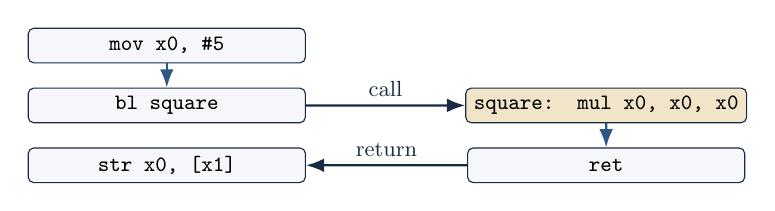
\begin{tikzpicture}[
  scale=.88,
  transform shape,
  node distance=.35cm,
  inst/.style={
    draw=navy,
    fill=softgray,
    rounded corners=2pt,
    minimum width=4.0cm,
    minimum height=.50cm,
    align=center,
    font=\small\ttfamily
  },
  note/.style={font=\small,align=center}
]
\node[inst] (c1) {mov x0, \#5};
\node[inst,below=of c1] (c2) {bl square};
\node[inst,below=of c2] (c3) {str x0, [x1]};
\node[inst,right=2.3cm of c2,fill=gold!25]
  (f1) {square: mul x0, x0, x0};
\node[inst,below=of f1] (f2) {ret};

\draw[-{Latex},thick,deepblue] (c1.south) -- (c2.north);
\draw[-{Latex},thick,deepblue] (f1.south) -- (f2.north);
\draw[-{Latex},thick,navy]
  (c2.east) -- node[above,note]{call} (f1.west);
\draw[-{Latex},thick,navy]
  (f2.west) -- node[above,note]{return} (c3.east);
\end{tikzpicture}
\end{center}
\vspace{0cm}
\begin{block}{Control-Flow Rule}
The call target runs temporarily, then \code{ret} resumes execution
after the original \code{bl} instruction.
\end{block}
\end{frame}

% ============================================================
% Slide 8
% Slide Header: Link Register Hazard
% ============================================================
\begin{frame}{The Link Register Hazard}
\begin{block}{Why Non-Leaf Functions Need Care}
A function that calls another function will execute its own \code{bl}.
That new \code{bl} overwrites \code{x30}.
\end{block}
\vspace{0cm}
\begin{columns}[T,onlytextwidth]
\column{0.48\textwidth}
\begin{block}{Leaf Function}
\begin{itemize}
\item Calls no other function.
\item May return using the original \code{x30}.
\item May not need a stack frame.
\end{itemize}
\end{block}
\column{0.48\textwidth}
\begin{block}{Non-Leaf Function}
\begin{itemize}
\item Calls at least one function.
\item Must preserve its return address if needed later.
\item Commonly saves \code{x30} on the stack.
\end{itemize}
\end{block}
\end{columns}
\vspace{0.05cm}
\begin{block}{Practical Rule}
If a function uses \code{bl} and still needs its caller's return
address, it must save \code{x30} before the nested call.
\end{block}
\end{frame}

% ============================================================
% Slide 9
% Slide Header: Arguments and Return Values
% ============================================================
\sectiondivider{Section 02}{Arguments and Return Values}

% ============================================================
% Slide 10
% Slide Header: Integer Argument Registers
% ============================================================
\begin{frame}{Integer Argument Registers}
\begin{block}{AArch64 Procedure Call Standard}
The first eight ordinary integer or pointer arguments use
\code{x0}--\code{x7}; 32-bit values use the corresponding
\code{w0}--\code{w7} views.
\end{block}
\vspace{0.1cm}
\begin{center}
\small
\renewcommand{\arraystretch}{1.08}
\begin{tabular}{
  >{\raggedright\arraybackslash}m{2.3cm}
  >{\raggedright\arraybackslash}m{8.1cm}
}
\rowcolor{navy}
{\color{white}\bfseries Register} &
{\color{white}\bfseries Common role at a function call} \\
\rowcolor{softgray}
\code{x0}--\code{x7} &
Integer/pointer arguments; \code{x0} also holds a common return value. \\
\rowcolor{white}
\code{x8} &
Indirect result location in some ABI-defined cases. \\
\rowcolor{softgray}
\code{x9}--\code{x15} &
Temporary registers available for general use. \\
\rowcolor{white}
\code{x16}, \code{x17} &
Intra-procedure-call scratch registers used by veneers/linker-generated
code. \\
\rowcolor{softgray}
\code{x18} &
Platform register; portable code should not treat it as an ordinary
temporary. \\
\end{tabular}
\end{center}
\end{frame}

% ============================================================
% Slide 11
% Slide Header: Arguments Beyond the Register Limit
% ============================================================
\begin{frame}{Arguments Beyond the Register Limit}
\begin{columns}[T,onlytextwidth]
\column{0.53\textwidth}
\begin{block}{More Than Eight Arguments}
After \code{x0}--\code{x7} are assigned, additional integer or pointer
arguments are passed in memory through the stack.
\end{block}
\vspace{0.15cm}
\begin{itemize}
\item The caller creates the required argument area.
\item The first stacked argument begins at the incoming \code{sp}.
\item Later stacked arguments follow at ABI-defined aligned offsets.
\item The caller removes its outgoing argument area after the call.
\end{itemize}
\column{0.43\textwidth}
\begin{block}{Nine-Argument Shape}
\small
\code{// a1--a8 use x0--x7}\\[0.10cm]
\code{sub sp, sp, \#16}\\[0.10cm]
\code{str x9, [sp]}\\[0.10cm]
\code{bl combine9}\\[0.10cm]
\code{add sp, sp, \#16}
\end{block}
\vspace{0.12cm}
\small
Here \code{x9} temporarily holds the ninth argument before the caller
stores it at the incoming stack location for \code{combine9}.
\end{columns}
\end{frame}

% ============================================================
% Slide 12
% Slide Header: Return Values
% ============================================================
\begin{frame}{Return Values}
\begin{block}{Common Integer Return}
\large
\hspace{3.7cm}\code{x0 = return value}
\normalsize
\end{block}
\vspace{0.2cm}
\begin{itemize}
\item A simple integer or pointer return value is placed in \code{x0}.
\item Some larger or multi-register return values may use additional
ABI rules.
\item The caller reads the return value after the callee executes
\code{ret}.
\item If the caller needs an argument value after the call, it must
preserve it if the register is caller-saved.
\end{itemize}
\vspace{0.15cm}
\begin{block}{Example}
\large
\hspace{3.2cm}\code{bl abs\_value}\\[0.10cm]
\hspace{3.2cm}\code{str x0, [x20]}
\normalsize
\end{block}
\end{frame}

% ============================================================
% Slide 13
% Slide Header: Example Function Call
% ============================================================
\begin{frame}{Example Function Call}
\begin{columns}[T,onlytextwidth]
\column{0.43\textwidth}
\begin{block}{C}
\large
\hspace{0.8cm}\code{z = add2(a, b);}
\normalsize
\end{block}
\vspace{0.15cm}
\begin{itemize}
\item First argument: \code{a}
\item Second argument: \code{b}
\item Return value assigned to \code{z}
\end{itemize}
\column{0.53\textwidth}
\begin{block}{AArch64 Shape}
\large
\hspace{0.8cm}\code{mov x0, x19}\\[0.10cm]
\hspace{0.8cm}\code{mov x1, x20}\\[0.10cm]
\hspace{0.8cm}\code{bl add2}\\[0.10cm]
\hspace{0.8cm}\code{mov x21, x0}
\normalsize
\end{block}
\vspace{0.15cm}
\small
The example assumes \code{a}, \code{b}, and \code{z} are being kept
in \code{x19}, \code{x20}, and \code{x21}.
\end{columns}
\end{frame}

% ============================================================
% Slide 14
% Slide Header: Simple Leaf Function
% ============================================================
\begin{frame}{Simple Leaf Function}
\begin{block}{C Function}
\large
\hspace{3.7cm}\code{long add2(long a, long b)}\\[0.10cm]
\hspace{3.7cm}\code{return a + b;}
\normalsize
\end{block}
\vspace{0.2cm}
\begin{block}{AArch64 Function Body}
\large
\hspace{3.7cm}\code{add2:}\\[0.10cm]
\hspace{3.7cm}\code{add x0, x0, x1}\\[0.10cm]
\hspace{3.7cm}\code{ret}
\normalsize
\end{block}
\vspace{0.15cm}
\begin{itemize}
\item \code{x0} and \code{x1} arrive holding the two arguments.
\item The sum is written to \code{x0}, the return-value register.
\item No stack frame is required for this simple leaf function.
\end{itemize}
\end{frame}

% ============================================================
% Slide 15
% Slide Header: Register Preservation
% ============================================================
\sectiondivider{Section 03}{Register Preservation Rules}

% ============================================================
% Slide 16.a
% Slide Header: AAPCS64 Is the Procedure-Call Blueprint
% ============================================================
\begin{frame}{AAPCS64 Is the Procedure-Call Blueprint}
\begin{block}{Arm Procedure Call Standard for AArch64}
AAPCS64 is the engineering blueprint that lets assembly routines,
compilers, libraries, linkers, and debuggers cooperate correctly.
\end{block}
\vspace{0cm}
\begin{columns}[T,onlytextwidth]
\column{0.48\textwidth}
\begin{block}{The Blueprint Defines}
\begin{itemize}
\item where arguments and results are placed
\item which registers may change or must be preserved
\item how \code{sp} and stack data are aligned
\end{itemize}
\end{block}
\column{0.48\textwidth}
\begin{block}{Why the Rules Matter}
\begin{itemize}
\item independently produced code can interoperate
\item callers and callees know their responsibilities
\item violations can corrupt data or return control
\end{itemize}
\end{block}
\end{columns}
\vspace{0cm}
\key{Two layers:} The A64 ISA defines what instructions can do;
AAPCS64 defines how software must use those capabilities at
procedure boundaries.
\end{frame}

% ============================================================
% Slide 16.b
% Slide Header: Caller-Saved and Callee-Saved Registers
% ============================================================
\begin{frame}{Caller-Saved and Callee-Saved Registers}
\begin{center}
\small
\renewcommand{\arraystretch}{1.05}
\begin{tabular}{
  >{\raggedright\arraybackslash}m{2.4cm}
  >{\raggedright\arraybackslash}m{2.7cm}
  >{\raggedright\arraybackslash}m{5.8cm}
}
\rowcolor{navy}
{\color{white}\bfseries Category} &
{\color{white}\bfseries Registers} &
{\color{white}\bfseries Meaning} \\
\rowcolor{softgray}
Caller-saved &
\code{x0}--\code{x17} &
A call may overwrite them; the caller saves live values it still needs. \\
\rowcolor{white}
Callee-saved &
\code{x19}--\code{x28} &
The callee must restore these before returning if it changes them. \\
\rowcolor{softgray}
Platform register &
\code{x18} &
Its use is platform-specific; portable code should avoid it. \\
\rowcolor{white}
Frame pointer &
\code{x29} &
Preserved when used as the current frame pointer. \\
\rowcolor{softgray}
Link register &
\code{x30} &
Holds the return address after \code{bl}; non-leaf functions commonly
save it. \\
\end{tabular}
\end{center}
\vspace{0.1cm}
\begin{block}{Core Distinction}
Caller-saved values may be destroyed by a call; callee-saved values
must be restored by the function that changes them.
\end{block}
\end{frame}

% ============================================================
% Slide 17.a
% Slide Header: A libc Call Uses the Same AAPCS64 Contract
% ============================================================
\begin{frame}{A libc Call Uses the Same AAPCS64 Contract}
\key{C call with nine total arguments:}\quad
\code{printf(format, v1, v2, \ldots, v8);}
\vspace{0.15cm}
\begin{columns}[T,onlytextwidth]
\column{0.43\textwidth}
\begin{block}{AAPCS64 Placement}
\small
\renewcommand{\arraystretch}{1.10}
\begin{tabular}{
  >{\raggedright\arraybackslash}m{1.50cm}
  >{\raggedright\arraybackslash}m{3.00cm}
}
\rowcolor{navy}
{\color{white}\bfseries Location} &
{\color{white}\bfseries Arg. or result} \\
\rowcolor{softgray}
\code{x0} &
address of \code{format} \\
\rowcolor{white}
\code{x1}--\code{x7} &
values \code{v1}--\code{v7} \\
\rowcolor{softgray}
\code{[sp]} &
\code{v8}: ninth total argument \\
\rowcolor{white}
\code{w0} &
characters printed on return \\
\end{tabular}
\end{block}
\column{0.53\textwidth}
\begin{block}{Caller Setup}
\small
\code{// x19 = format; x20--x27 = v1--v8}\\[0.06cm]
\code{sub sp, sp, \#16}\\[0.045cm]
\code{str x27, [sp]}\quad\code{// v8}\\[0.045cm]
\code{mov x0, x19}\quad\code{// format}\\[0.045cm]
\code{mov x1, x20}\quad\code{// v1}\\[0.045cm]
\code{// repeat through x7 = v7}\\[0.045cm]
\code{bl printf}\\[0.045cm]
\code{add sp, sp, \#16}
\end{block}
\end{columns}
\vspace{0.08cm}
\small
\key{Why it works:} libc finds every argument because both sides
follow AAPCS64. The surrounding non-leaf function preserves
\code{x30} separately.
\end{frame}

% ============================================================
% Slide 17.b
% Slide Header: Caller-Saved Example
% ============================================================
\begin{frame}{Caller-Saved Example}
\begin{block}{Situation}
The caller has a live value in \code{x0}, but also needs to call
another function. Since \code{x0} is caller-saved, the caller must
protect it if the value is still needed.
\end{block}
\vspace{0.2cm}
\large
\hspace{3.1cm}\code{str x0, [sp, \#-16]!}\\[0.10cm]
\hspace{3.1cm}\code{bl helper}\\[0.10cm]
\hspace{3.1cm}\code{ldr x1, [sp], \#16}
\normalsize
\vspace{0.2cm}
\begin{itemize}
\item This example reserves 16 bytes to preserve stack alignment.
\item The result from \code{helper} remains in \code{x0}; the saved
value is restored into \code{x1}.
\item The principle is that the caller saves caller-saved values it
still needs.
\end{itemize}
\end{frame}

% ============================================================
% Slide 18
% Slide Header: Callee-Saved Example
% ============================================================
\begin{frame}{Callee-Saved Example}
\begin{block}{Situation}
A function wants to use \code{x19}. Because \code{x19} is
callee-saved, the function must restore the caller's original
\code{x19} before returning.
\end{block}
\vspace{0.15cm}
\large
\hspace{3.2cm}\code{str x19, [sp, \#-16]!}\\[0.10cm]
\hspace{3.2cm}\code{// use x19 inside function}\\[0.10cm]
\hspace{3.2cm}\code{ldr x19, [sp], \#16}\\[0.10cm]
\hspace{3.2cm}\code{ret}
\normalsize
\vspace{0.15cm}
\begin{block}{Preservation Rule}
The caller should see the same \code{x19} value after the function
returns as before the call began.
\end{block}
\end{frame}

% ============================================================
% Slide 19
% Slide Header: Common Register Roles
% ============================================================
\begin{frame}{Common Register Roles}
\begin{center}
\small
\renewcommand{\arraystretch}{1.03}
\begin{tabular}{
  >{\raggedright\arraybackslash}m{2.6cm}
  >{\raggedright\arraybackslash}m{8.5cm}
}
\rowcolor{navy}
{\color{white}\bfseries Register(s)} &
{\color{white}\bfseries Typical ABI role} \\
\rowcolor{softgray}
\code{x0}--\code{x7} &
Integer/pointer arguments and return values. \\
\rowcolor{white}
\code{x9}--\code{x15} &
Temporary caller-saved registers. \\
\rowcolor{softgray}
\code{x16}, \code{x17} &
Intra-procedure-call temporaries; veneers may overwrite them. \\
\rowcolor{white}
\code{x18} &
Platform register with platform-specific use. \\
\rowcolor{softgray}
\code{x19}--\code{x28} &
Callee-saved registers. \\
\rowcolor{white}
\code{x29} &
Frame pointer, when a frame pointer is used. \\
\rowcolor{softgray}
\code{x30} &
Link register, holding a return address after \code{bl}. \\
\rowcolor{white}
\code{sp} &
Stack pointer; 16-byte aligned at public interfaces and when used for
memory access. \\
\end{tabular}
\end{center}
\end{frame}

% ============================================================
% Slide 20
% Slide Header: Stack Frames
% ============================================================
\sectiondivider{Section 04}{Stack Frames}

% ============================================================
% Slide 21
% Slide Header: The Stack Grows Down
% ============================================================
\begin{frame}{The Stack Grows Down}
\begin{columns}[T,onlytextwidth]
\column{0.52\textwidth}
\begin{itemize}
\item The stack is a memory region used for call-related temporary
storage.
\item Under AAPCS64, \code{sp} is 16-byte aligned at public interfaces
and whenever memory is accessed through \code{sp}.
\item Pushing data usually subtracts from \code{sp}.
\item Popping data usually adds back to \code{sp}.
\end{itemize}
\vspace{0.15cm}
\begin{block}{Direction}
The stack grows toward lower addresses, so allocating stack space
means decreasing \code{sp}.
\end{block}
\column{0.42\textwidth}
\begin{center}
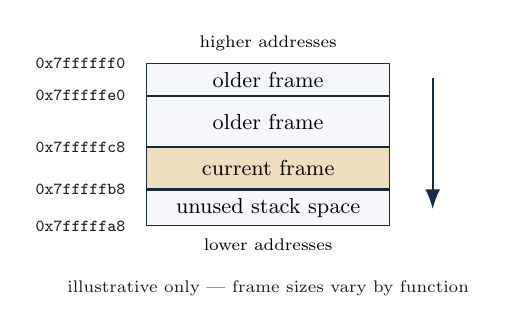
\begin{tikzpicture}[
  scale=.87,
  transform shape,
  region/.style={
    draw=navy,
    minimum width=3.55cm,
    align=center,
    font=\small
  },
  used/.style={region,fill=softgray},
  cur/.style={region,fill=gold!30},
  addr/.style={
    font=\scriptsize\ttfamily,
    anchor=east,
    text=darkgray
  }
]
\node[font=\scriptsize] (hi) {higher addresses};

\node[used,minimum height=.46cm,below=.06cm of hi]
  (old1) {older frame};
\node[used,minimum height=.74cm,below=0pt of old1]
  (old2) {older frame};
\node[cur,minimum height=.60cm,below=0pt of old2]
  (curf) {current frame};
\node[used,minimum height=.52cm,below=0pt of curf]
  (free) {unused stack space};
\node[font=\scriptsize,below=.06cm of free]
  (lo) {lower addresses};

\node[addr,left=.18cm of old1.north west] {0x7ffffff0};
\node[addr,left=.18cm of old1.south west] {0x7fffffe0};
\node[addr,left=.18cm of old2.south west] {0x7fffffc8};
\node[addr,left=.18cm of curf.south west] {0x7fffffb8};
\node[addr,left=.18cm of free.south west] {0x7fffffa8};

\draw[-{Latex[length=2.5mm]},thick,navy]
  ([xshift=.62cm,yshift=.02cm]old1.east)
  --
  ([xshift=.62cm,yshift=-.02cm]free.east);

\node[
  font=\scriptsize,
  text=darkgray,
  align=center,
  below=.20cm of lo
] {illustrative only --- frame sizes vary by function};
\end{tikzpicture}
\end{center}
\end{columns}
\end{frame}

% ============================================================
% Slide 22
% Slide Header: Stack Frame Contents
% ============================================================
\begin{frame}{Stack Frame Contents}
\begin{columns}[T,onlytextwidth]
\column{0.50\textwidth}
\begin{itemize}
\item Saved return address when \code{x30} must be preserved.
\item Saved frame pointer when \code{x29} is used.
\item Saved callee-saved registers used by the function.
\item Local variables or spill slots that do not fit in registers.
\item Outgoing stack arguments when register arguments are insufficient.
\end{itemize}
\column{0.46\textwidth}
\begin{center}
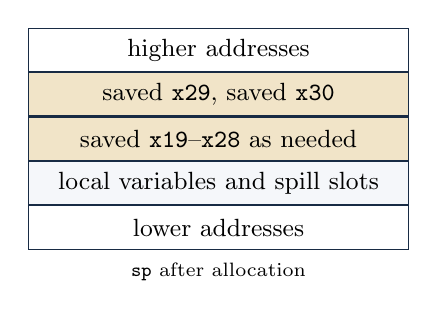
\begin{tikzpicture}[
  row/.style={
    draw=navy,
    text width=4.6cm,
    minimum height=.55cm,
    align=center,
    font=\small
  },
  saved/.style={row,fill=gold!25},
  local/.style={row,fill=softgray}
]
\node[row,fill=white] (top) {higher addresses};
\node[saved,below=0pt of top]
  (lr) {saved \code{x29}, saved \code{x30}};
\node[saved,below=0pt of lr]
  (regs) {saved \code{x19}--\code{x28} as needed};
\node[local,below=0pt of regs]
  (loc) {local variables and spill slots};
\node[row,fill=white,below=0pt of loc]
  (bot) {lower addresses};
\node[font=\scriptsize,below=.05cm of bot]
  {\code{sp} after allocation};
\end{tikzpicture}
\end{center}
\end{columns}
\end{frame}

% ============================================================
% Slide 23
% Slide Header: Function Prologue
% ============================================================
\begin{frame}{Function Prologue}
\begin{block}{Purpose}
A prologue prepares the callee's execution environment before the
function body runs.
\end{block}
\vspace{0.2cm}
\large
\hspace{3.0cm}\code{stp x29, x30, [sp, \#-16]!}\\[0.10cm]
\hspace{3.0cm}\code{mov x29, sp}
\normalsize
\vspace{0.2cm}
\begin{itemize}
\item The first instruction allocates 16 bytes and stores old
\code{x29} and \code{x30}.
\item \code{mov x29, sp} establishes a frame pointer for this frame.
\item Additional stack allocation may follow if locals or spills are
needed.
\end{itemize}
\vspace{0.15cm}
\begin{block}{Compiler Variation}
Depending on the platform ABI profile and optimization choices, code
may omit \code{x29} as a frame pointer or use a different frame layout
while preserving its obligations.
\end{block}
\end{frame}

% ============================================================
% Slide 24
% Slide Header: Function Epilogue
% ============================================================
\begin{frame}{Function Epilogue}
\begin{block}{Purpose}
An epilogue restores the caller's environment before returning.
\end{block}
\vspace{0.2cm}
\large
\hspace{3.0cm}\code{ldp x29, x30, [sp], \#16}\\[0.10cm]
\hspace{3.0cm}\code{ret}
\normalsize
\vspace{0.2cm}
\begin{itemize}
\item The load pair restores the previous frame pointer and return
address.
\item Post-indexing adds 16 to \code{sp}, releasing the stack space.
\item \code{ret} branches to the restored return address in \code{x30}.
\end{itemize}
\vspace{0.15cm}
\begin{block}{Stack Balance}
A function that subtracts from \code{sp} must add the same amount back
before returning.
\end{block}
\end{frame}

% ============================================================
% Slide 25
% Slide Header: Prologue and Epilogue Diagram
% ============================================================
\begin{frame}{Prologue and Epilogue Diagram}
\begin{center}
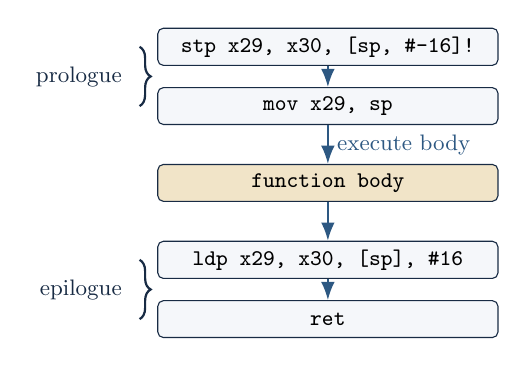
\begin{tikzpicture}[
  scale=.90,
  transform shape,
  inst/.style={
    draw=navy,
    fill=softgray,
    rounded corners=2pt,
    minimum width=4.8cm,
    minimum height=.52cm,
    align=center,
    font=\small\ttfamily
  },
  note/.style={font=\small,align=center}
]
\node[inst] (a) {stp x29, x30, [sp, \#-16]!};
\node[inst,below=.30cm of a] (b) {mov x29, sp};
\node[inst,below=.55cm of b,fill=gold!25]
  (c) {function body};
\node[inst,below=.55cm of c]
  (d) {ldp x29, x30, [sp], \#16};
\node[inst,below=.30cm of d] (e) {ret};

\draw[-{Latex},thick,deepblue] (a.south) -- (b.north);
\draw[-{Latex},thick,deepblue]
  (b.south) -- node[right,note]{execute body} (c.north);
\draw[-{Latex},thick,deepblue] (c.south) -- (d.north);
\draw[-{Latex},thick,deepblue] (d.south) -- (e.north);

\draw[
  decorate,
  decoration={brace,amplitude=4pt},
  thick,
  navy
]
  ([xshift=-.25cm]a.west)
  --
  ([xshift=-.25cm]b.west)
  node[midway,left=.12cm,font=\small]{prologue};

\draw[
  decorate,
  decoration={brace,amplitude=4pt},
  thick,
  navy
]
  ([xshift=-.25cm]d.west)
  --
  ([xshift=-.25cm]e.west)
  node[midway,left=.12cm,font=\small]{epilogue};
\end{tikzpicture}
\end{center}
\vspace{-0.05cm}
\begin{block}{Function Entry and Exit}
The prologue establishes the function's stack-frame state before the
body executes. The epilogue reverses those changes, restores the saved
return state, and then \code{ret} transfers control back to the caller.
\end{block}
\end{frame}

% ============================================================
% Slide 26
% Slide Header: Local Stack Storage
% ============================================================
\begin{frame}{Local Stack Storage}
\begin{block}{When Registers Are Not Enough}
A function may allocate additional stack space for local arrays,
temporary spill slots, or values whose address must be taken.
\end{block}
\vspace{0.15cm}
\large
\hspace{2.8cm}\code{sub sp, sp, \#32}\\[0.10cm]
\hspace{2.8cm}\code{str x0, [sp, \#16]}\\[0.10cm]
\hspace{2.8cm}\code{ldr x1, [sp, \#16]}\\[0.10cm]
\hspace{2.8cm}\code{add sp, sp, \#32}
\normalsize
\vspace{0.15cm}
\begin{itemize}
\item Stack space is usually allocated in multiples that preserve
alignment.
\item Positive offsets from \code{sp} or \code{x29} can address slots
in the frame.
\item The frame layout is a compiler convention, not an A64
instruction requirement.
\end{itemize}
\end{frame}

% ============================================================
% Slide 27
% Slide Header: Leaf and Non-Leaf Functions
% ============================================================
\sectiondivider{Section 05}{Function Calls and Recursion}

% ============================================================
% Slide 28
% Slide Header: Leaf Function without a Stack Frame
% ============================================================
\begin{frame}{Leaf Function without a Stack Frame}
\begin{block}{Leaf Function}
A leaf function calls no other function. If it only uses caller-saved
registers and needs no local stack storage, it may avoid stack use
entirely.
\end{block}
\vspace{0.2cm}
\large
\hspace{3.6cm}\code{double\_it:}\\[0.10cm]
\hspace{3.6cm}\code{add x0, x0, x0}\\[0.10cm]
\hspace{3.6cm}\code{ret}
\normalsize
\vspace{0.2cm}
\begin{itemize}
\item Argument arrives in \code{x0}.
\item Return value is written back into \code{x0}.
\item \code{x30} is not overwritten because this function makes no
nested calls.
\end{itemize}
\end{frame}

% ============================================================
% Slide 29
% Slide Header: Non-Leaf Function Saves the Link Register
% ============================================================
\begin{frame}{Non-Leaf Function Saves the Link Register}
\begin{block}{Nested Call}
A non-leaf function must preserve its own return address before
executing another \code{bl} if it needs to return to its caller
afterward.
\end{block}
\vspace{0.15cm}
\small
\hspace{3.0cm}\code{outer:}\\[0.08cm]
\hspace{3.0cm}\code{stp x29, x30, [sp, \#-16]!}\\[0.08cm]
\hspace{3.0cm}\code{mov x29, sp}\\[0.08cm]
\hspace{3.0cm}\code{bl inner}\\[0.08cm]
\hspace{3.0cm}\code{add x0, x0, \#1}\\[0.08cm]
\hspace{3.0cm}\code{ldp x29, x30, [sp], \#16}\\[0.08cm]
\hspace{3.0cm}\code{ret}
\normalsize
\vspace{0.15cm}
\begin{block}{Reason}
The \code{bl inner} instruction overwrites \code{x30}; therefore
\code{outer} saves its original \code{x30} first.
\end{block}
\end{frame}

% ============================================================
% Slide 30
% Slide Header: Recursion Requires Separate Frames
% ============================================================
\begin{frame}{Recursion Requires Separate Frames}
\begin{block}{Recursive Calls}
Each recursive call needs its own preserved state: return address,
saved registers, and local values that must survive the nested call.
\end{block}
\vspace{0.2cm}
\begin{columns}[T,onlytextwidth]
\column{0.50\textwidth}
\begin{itemize}
\item One invocation cannot reuse another invocation's saved return
address.
\item Local variables from different recursion depths must remain
distinct.
\item Stack frames naturally provide separate storage per invocation.
\end{itemize}
\column{0.46\textwidth}
\begin{center}
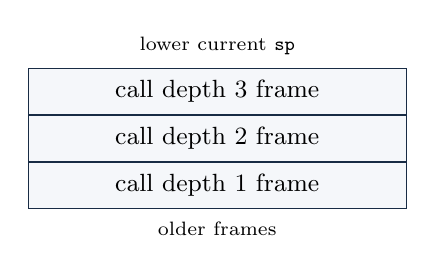
\begin{tikzpicture}[
  framebox/.style={
    draw=navy,
    minimum width=4.8cm,
    minimum height=.58cm,
    align=center,
    font=\small,
    fill=softgray
  }
]
\node[framebox] (f3) {call depth 3 frame};
\node[framebox,below=0pt of f3] (f2) {call depth 2 frame};
\node[framebox,below=0pt of f2] (f1) {call depth 1 frame};
\node[font=\scriptsize,above=.05cm of f3]
  {lower current \code{sp}};
\node[font=\scriptsize,below=.05cm of f1]
  {older frames};
\end{tikzpicture}
\end{center}
\end{columns}
\end{frame}

% ============================================================
% Slide 31
% Slide Header: Recursive Factorial Uses One Frame per Call
% ============================================================
\begin{frame}{Recursive Factorial Uses One Frame per Call}
\begin{columns}[T,onlytextwidth]
\column{0.48\textwidth}
\begin{block}{Entry and Base Case}
\small
\code{fact:}\\[0.08cm]
\code{stp x29, x30, [sp, \#-32]!}\\[0.08cm]
\code{mov x29, sp}\\[0.08cm]
\code{str x0, [sp, \#16]}\\[0.08cm]
\code{cmp x0, \#1}\\[0.08cm]
\code{b.gt recurse}\\[0.08cm]
\code{mov x0, \#1}\\[0.08cm]
\code{b done}
\end{block}
\column{0.48\textwidth}
\begin{block}{Recursive Case and Return}
\small
\code{recurse:}\\[0.08cm]
\code{sub x0, x0, \#1}\\[0.08cm]
\code{bl fact}\\[0.08cm]
\code{ldr x1, [sp, \#16]}\\[0.08cm]
\code{mul x0, x1, x0}\\[0.08cm]
\code{done:}\\[0.08cm]
\code{ldp x29, x30, [sp], \#32}\\[0.08cm]
\code{ret}
\end{block}
\end{columns}
\vspace{0.10cm}
\small
Each invocation preserves its return address and original \code{n};
the recursive result returns in \code{x0}.
\end{frame}

% ============================================================
% Slide 32
% Slide Header: Common Procedure Bugs
% ============================================================
\begin{frame}{Common Procedure Bugs}
\begin{itemize}
\item Forgetting that \code{bl} overwrites \code{x30}.
\item Changing \code{x19}--\code{x28} without restoring them before
returning.
\item Returning with \code{sp} different from its value at function
entry.
\item Assuming caller-saved registers survive a call.
\item Using \code{w} registers for pointer values that require 64-bit
addresses.
\item Adjusting \code{sp} by only 8 bytes and then accessing memory
through the misaligned stack pointer.
\end{itemize}
\vspace{0.15cm}
\begin{block}{Debugging Order}
Check the return address, then stack balance, then
register-preservation rules.
\end{block}
\end{frame}

% ============================================================
% Slide 33
% Slide Header: Summary and Self-Test
% ============================================================
\sectiondivider{Section 06}{Summary and Self-Test}

% ============================================================
% Slide 34
% Slide Header: Topic 8 Summary
% ============================================================
\begin{frame}{Topic 8 Summary}
\begin{itemize}
\item \code{bl} calls a function and writes the return address into
\code{x30}.
\item \code{ret} returns to the address held in \code{x30} by default.
\item \code{x0}--\code{x7} pass the first eight integer/pointer
arguments; 32-bit values use \code{w0}--\code{w7}.
\item Additional arguments use the stack, and \code{x0} holds a common
integer/pointer return value.
\item Caller-saved registers may be overwritten by a call; callee-saved
registers must be restored if changed.
\item Stack frames preserve return addresses, saved registers, and
local storage.
\item Leaf functions may avoid stack frames; non-leaf and recursive
functions often need them.
\end{itemize}
\end{frame}

% ============================================================
% Slide 35
% Slide Header: Self-Test 1/2
% ============================================================
\begin{frame}{Self-Test 1/2}
\begin{enumerate}
\item What does \code{bl function} write into \code{x30}?
\item Why can a non-leaf function not blindly trust \code{x30} after
it calls another function?
\item Which registers carry the first eight integer or pointer
arguments, and where is a ninth argument passed?
\item Where is a simple integer return value normally placed?
\item What is the difference between caller-saved and callee-saved
registers?
\end{enumerate}
\end{frame}

% ============================================================
% Slide 36
% Slide Header: Self-Test 2/2
% ============================================================
\begin{frame}{Self-Test 2/2}
\begin{enumerate}
\setcounter{enumi}{5}
\item Why does \code{stp x29, x30, [sp, \#-16]!} both allocate stack
space and save registers?
\item What does \code{ldp x29, x30, [sp], \#16} do before the final
\code{ret}?
\item Why must \code{sp} be restored before returning to the caller?
\item Why can a small leaf function sometimes avoid a stack frame?
\item Why does recursion require a separate stack frame for each
active call?
\end{enumerate}
\end{frame}

% ============================================================
% Slide 37
% Slide Header: Register Preservation Exercise
% ============================================================
\begin{frame}{Register Preservation Exercise}
\begin{block}{Classify Each Register}
For each register, state whether it is mainly used for argument/return,
caller-saved temporary use, callee-saved preservation, frame pointer,
link register, or stack pointer.
\end{block}
\vspace{0.15cm}
\begin{center}
\small
\renewcommand{\arraystretch}{1.16}
\begin{tabular}{
  >{\raggedright\arraybackslash}m{4.0cm}
  >{\raggedright\arraybackslash}m{6.4cm}
}
\rowcolor{navy}
{\color{white}\bfseries Register} &
{\color{white}\bfseries Classification} \\
\rowcolor{softgray}
\code{x0} & \\
\rowcolor{white}
\code{x9} & \\
\rowcolor{softgray}
\code{x19} & \\
\rowcolor{white}
\code{x29} & \\
\rowcolor{softgray}
\code{x30} & \\
\rowcolor{white}
\code{sp} & \\
\end{tabular}
\end{center}
\end{frame}

% ============================================================
% Slide 38
% Slide Header: Next Topic
% ============================================================
\begin{frame}{Next Topic}
\begin{block}{Machine Instruction Encoding}
Topic 9 moves from assembly-level procedure structure to the binary
encoding of selected A64 instructions.
\end{block}
\vspace{0.25cm}
\begin{itemize}
\item AArch64 instruction formats and machine-code fields
\item Data-processing instruction encoding
\item Memory instruction encoding and PC-relative addressing
\item Branch instruction encoding and machine-code decoding
\end{itemize}
\end{frame}

\end{document}